% Title : hw9
% Author: Bhishan Poudel
% Date  : Oct 31, 2015


\documentclass[11pt,a4paper,english]{article}
\usepackage{babel}
\usepackage{amsmath}
\usepackage{amssymb}
\usepackage{graphicx,subfigure}
\usepackage[export]{adjustbox}    % for positioning figure
\usepackage{textcomp}
\usepackage{fixltx2e}
\usepackage[usenames,dvipsnames,svgnames,table]{xcolor}

% some useful newcommands
\newcommand{\nl}{\nonumber \\}
\newcommand{\no}{\nonumber}
\newcommand{\ul}{\underline}
\newcommand{\ol}{\overline}

%some useful newcommands
\newcommand{\beq}{\begin{equation}}
\newcommand{\eeq}{\end{equation}}
\newcommand{\bfig}{\begin{figure}}
\newcommand{\efig}{\end{figure}}
\newcommand{\beqa}{\begin{eqnarray}}
\newcommand{\eeqa}{\end{eqnarray}}
\newcommand{\beqan}{\begin{eqnarray*}}
\newcommand{\eeqan}{\end{eqnarray*}}
\newcommand{\ba}{\begin{array}}
\newcommand{\ea}{\end{array}}
\newcommand{\ben}{\begin{enumerate}}
\newcommand{\een}{\end{enumerate}}
\newcommand{\bfl}{\begin{flushleft}}
\newcommand{\efl}{\end{flushleft}}
\newcommand{\btab}{\begin{tabular}}
\newcommand{\etab}{\end{tabular}}
\newcommand{\bit}{\begin{itemize}}
\newcommand{\eit}{\end{itemize}}
\newcommand{\bdes}{\begin{description}}
\newcommand{\edes}{\end{description}}
\newcommand{\bdm}{\begin{displaymath}}
\newcommand{\edm}{\end{displaymath}}
\newcommand {\IR} [1]{\textcolor{red}{#1}}

% for listing
\usepackage{enumitem}
\usepackage[ampersand]{easylist}
\ListProperties(Hide=100, Hang=true, Progressive=3ex, Style*=-- ,
Style2*=$\bullet$ ,Style3*=$\circ$ ,Style4*=\tiny$\blacksquare$ )    % for easylist
\newcommand{\begl}{\begin{easylist}}
\newcommand{\eegl}{\end{easylist}}

% for hyperlink
\usepackage{hyperref}             % for hyperlink
\hypersetup{
    colorlinks=true,
    linkcolor=blue,
    filecolor=magenta,      
    urlcolor=cyan,    
    bookmarks=true
    }


% Creating Title for the assessment

\title{Homework 9: Monte Carlo Application}
\author{Bhishan Poudel}
\date{Oct 31,2015}

% to avoid indentation in paragraphs
\usepackage[parfill]{parskip}

% begin of document
\begin{document}
\maketitle
\tableofcontents
\listoffigures
\clearpage

%%%%%%%%%%%%%%%%%%%%%%%%%%%%%%%%%%%%%%%%%%%%%%%%%%%%%%%%%%%%%%%%%%%%%%%%%%%%%%%%%%%%%%%%%%%%%%%%%%%%%

\section{Question 1: Multi-dimensional integration }
In this question I evaluated the $10$ dimensional integration and checked with the analytic result. 

	The solution directory is :\\
	\begin{verbatim}
	location             : hw9/qn1
	provided code        : int_10d.f90
	source code          : hw9qn1.f90
	datafiles            : hw9qn1b.dat and hw9qn1c.dat
	plots                : hw9qn1c.eps
	\end{verbatim}
	
	\subsection{part : a }	
	I conducted $16$ trials and took the average value as the result.
		
	\subsection{part : b }
    I took the sample sizes $N = 2,4,8,...,8196$
	
	\subsection{part : c }
    I plotted the graph for absolute error vs. $1/\sqrt{N}$ and did a linear fit. 

	
	    The figures are shown below:\\
    %%%% including figure %%%%%%%%%%%%%%%%%%
	\begin{figure}[h!]
	\centering
	\includegraphics [scale=0.6]{figures/hw9qn1c.eps}
	\caption{Plot of absolute error vs. $1/\sqrt{N}$ }
	\end{figure}
	\clearpage
	%%%%%%%%%%%%%%%%%%%%%%%%%%%%%%%%%%%%%%%		
%%%%%%%%%%%%%%%%%%%%%%%%%%%%%%%%%%%%%%%%%%%%%%%%%%%%%%%%%%%%%%%%%%%%%%%%%%%%%%%%%%%%%%%%%
\section{Question 2: $3$D Integration with Importance Sampling  }

	In this question I evaluated the given three dimensional integral using :\\
	a) function 'drand', without importance sampling.\\
	b) function 'drand', with importance sampling.\\
	c) subroutine 'sobseq' with importance sampling.\\
	d) using gaussian quadrature (gauleg) integration method.\\	
   	
	\subsection{part a: $3$d integral using in built function 'drand', without importance sampling }
	
	In this part I used built in random number generator 'drand' to evaluate the given three
	dimensional integral. I took 16 trials and plotted the answer as function of $1/\sqrt{N}$.
	I found that converged result is $0.37$.\\
	
			The solution directory is :\\
	\begin{verbatim}
	location             : hw9/qn2/2a
	provided code        : int_10d.f90
	source code          : hw9qn2a.f90
	datafiles            : hw9qn2a.dat
	plots                : hw9qn2a.eps
	\end{verbatim}
	
		    The figures are shown below:\\
    %%%% including figure %%%%%%%%%%%%%%%%%%
	\begin{figure}[h!]
	\centering
	\includegraphics [scale=0.6,angle=270]{figures/hw9qn2a.eps}
	\caption{Plot of integral vs. $1/\sqrt{N}$ }
	\end{figure}
	\clearpage
	%%%%%%%%%%%%%%%%%%%%%%%%%%%%%%%%%%%%%%%

%%%%%%%%%%%%%%%%%%%%%%%%%%%%%%%%%%%%%%%%%%%%%%%%%%%%%%%%%%%%%%%%%%%%%%%%%%%%%%%%	
\subsection{part b: integration using drand and importance sampling}
In this part I evaluated the integral using built-in function 'drand' and also used
importance sampling. I used tangent map for $x$ integral and logarithmic map
for $y$ and $z$ integrals.
It took sample size $n=64$ to reach the answer $0.37$.\\
I plotted the graph of $\frac{1}{\sqrt{N}}$ vs. $result$

			The solution directory is :\\
	\begin{verbatim}
	location             : hw9/qn2/2b
	provided code        : int_10d.f90, log_car_sob.f90
	source code          : hw9qn2b.f90
	datafiles            : hw9qn2b.dat
	gnuplot file         : hw9qn2b.gp
	plots                : hw9qn2b.eps
	\end{verbatim}
	
		    The figures are shown below:\\
    %%%% including figure %%%%%%%%%%%%%%%%%%
	\begin{figure}[h!]
	\centering
	\includegraphics [scale=0.6]{figures/hw9qn2b.eps}
	\caption{Plot of integral vs. $1/\sqrt{N}$ }
	\end{figure}
	\clearpage
	%%%%%%%%%%%%%%%%%%%%%%%%%%%%%%%%%%%%%%%

%%%%%%%%%%%%%%%%%%%%%%%%%%%%%%%%%%%%%%%%%%%%%%%%%%%%%%%%%%%%%%%%%%%%%%%%%%%%%%%%
%%%%%%%%%%%%%%%%%%%%%%%%%%%%%%%%%%%%%%%%%%%%%%%%%%%%%%%%%%%%%%%%%%%%%%%%%%%%%%%%	
\subsection{part c: integration using sobol sequence and importance sampling}
In this part I evaluated the integral using given subroutine 'sobseq' and also used
importance sampling. I used tangent map for $x$ integral and logarithmic map
for $y$ and $z$ integrals.
It took sample size $n=1024$ to reach the answer $0.37$.\\
I plotted the graph of $\frac{1}{N}$ vs. $result$.
I also compared cpu-time for method using `drand' and `sobseq', I found that
`sobseq' is slower. We can see the computation time in part $2d$.\\

			The solution directory is :\\
	\begin{verbatim}
	location             : hw9/qn2/2c
	provided code        : int_10d.f90, log_car_sob.f90
	source code          : hw9qn2c.f90
	datafiles            : hw9qn2c.dat
	gnuplot file         : hw9qn2c.gp
	plots                : hw9qn2c.eps
	\end{verbatim}
	
		    The figures are shown below:\\
    %%%% including figure %%%%%%%%%%%%%%%%%%
	\begin{figure}[h!]
	\centering
	\includegraphics [scale=0.6]{figures/hw9qn2c.eps}
	\caption{Plot of integral vs. $1/N$ }
	\end{figure}
	\clearpage
	%%%%%%%%%%%%%%%%%%%%%%%%%%%%%%%%%%%%%%%

%%%%%%%%%%%%%%%%%%%%%%%%%%%%%%%%%%%%%%%%%%%%%%%%%%%%%%%%%%%%%%%%%%%%%%%%%%%%%%%%
\subsection{part d: $3$d integration using gaussian quadrature (gauleg) }
	
    In this part I calculated three integrals separately and multiplied them 
    to get the three dimensional integral.
    I also calcualted the error of each integrals in comparison to 'true'
    values given by Wolfram Alpha online.\\
    Comparing with Monte Carlo Importance Sampling, gaussian quadrature method
    is slow.\\
    The first integral is:\\
    
    \begin{eqnarray}
    I_{x} &=& \int \frac{1}{1 + x^{2}}  \,dx = tan^{-1}x + constant\\
    I_{x} &=& \int_{0}^{1} \!\! \frac{1}{1 + x^{2}}  \,dx = \pi/4 = 0.78540
    \end{eqnarray}
    
    The second integral is:\\
    
    \begin{eqnarray}
    I_{y} &=& \int ye^{-y^{2}}  \,dy = -\frac{e^{-y^{2}}}{2} + constant\\
    I_{y} &=& \int_{0}^{1} \!\! ye^{-y^{2}}  \,dy = 0.31606
    \end{eqnarray}
    
    The third integral is:\\
    
    \begin{eqnarray}
    I_{z} &=& \int \frac{e^{-z}} {\sqrt{z}}  \,dz = \sqrt{\pi} \quad erf(z) + constant\\
    I_{z} &=& \int_{0}^{1} \!\! \frac{e^{-z}} {\sqrt{z}}   \,dz = \sqrt{\pi} \quad erf(1) = 1.49365
    \end{eqnarray}
    
    I evaluated the integrals and errors separately and multiplied in the end.    
    Final result is $= 0.78540 * 0.31606 * 1.49365 = 0.37$
    
    		The solution directory is :\\
	\begin{verbatim}
	location             : hw9/qn2/2d
	provided codes       : gauleg.f90
	source code          : hw9qn2d.f90
	datafiles            : hw9qn2d.dat
	\end{verbatim}
%%%%%%%%%%%%%%%%%%%%%%%%%%%%%%%%%%%%%%%%%%%%%%%%%%%%%%%%%%%%%%%%%%%%%%%%%%%%%%%%	
	\subsection{part e: computation time}
	To find the cpu-time i used the bash command:\\
	time $./a.out$\\
	to find the cpu-time of computation.\\
	I found that integration with importance sampling was faster
	than without importance sampling and gaussian quadrature method.\\
	The cpu-time of computation is shown below.
	
	\begin{verbatim}
	
	For part 2a	 
    real	0m0.265s
    user	0m0.051s
    sys	    0m0.011s
    
    part 2b       
    real	0m0.009s
    user	0m0.005s
    sys	    0m0.005s
    
    part 2c
    real	0m0.045s
    user	0m0.040s
    sys	    0m0.008s
    
    part 2d
    real	0m0.098s
    user	0m0.094s
    sys	    0m0.004s
	
	\end{verbatim} 
    

\end{document}

